\documentclass[a4paper]{article}

\usepackage{microtype}
\usepackage{enumitem}
\usepackage{mathtools, amssymb, amsthm}
\usepackage{subcaption}
\usepackage{graphicx}
\usepackage{bbm}

\setlength{\parindent}{0em}

\title{4}
\date{}

\graphicspath{ {../images} }

\begin{document}
\maketitle

\subsection{MATLAB Plot}

Below, we can see the original image that was described in the question:
\begin{figure}[h]
\centering

\includegraphics[scale=0.5]{raw_img.png}
\caption{The original $201\times 201$ black image with a white row in the middle.}
\label{f:orig}
\end{figure}

A plot of the logarithm of the modulus of the DFT of the image can be found below:
\begin{figure}[h]
\centering
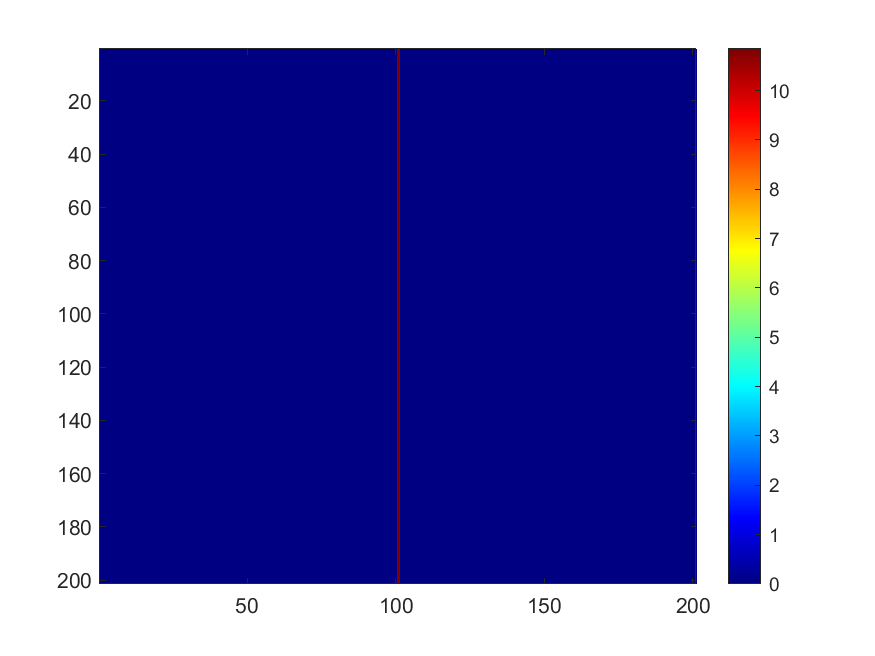
\includegraphics[scale=0.5]{fft.png}
\caption{The $\log$ plot of the modulus of the DFT of Figure (\ref{f:orig}).}
\end{figure}

\subsection{Analytical Derivation}

We know that the formula for the DFT of a 2D signal is as follows:
\begin{equation*}
F_d(u, v) = \dfrac{1}{\sqrt{W_1W_2}} \sum\limits_{x = 0}^{W_1 - 1} \sum\limits_{y = 0}^{W_2 - 1} f(x, y) \exp\left (-i2\pi \left (\dfrac{ux}{W_1} + \dfrac{vy}{W_2}\right )\right )
\end{equation*}

Since we know that in our image, $W_1 = W_2 = 201$, we can substitute this into the formula:
\begin{equation}
F_d(u, v) = \dfrac{1}{201} \sum\limits_{x = 0}^{200} \sum\limits_{y = 0}^{200} f(x, y) \exp\left (-i2\pi \left (\dfrac{ux}{201} + \dfrac{vy}{201}\right )\right )
\label{eq:dft}
\end{equation}

In our case, our 2D signal is the image shown in Figure \ref{f:orig}, and its definition is
\begin{equation*}
f(x, y) =
\begin{dcases}
0, y \in \{0, 1, 2, \dots, 200\} \text{ and } y \ne 100, & x \in \{0, 1, 2, \dots, 200\} \\
1, y = 100, & x \in \{0, 1, 2, \dots, 200\}
\end{dcases}
\end{equation*}

Observe that we normalized the image intensities, so the range of intensity values is $[0, 1]$, instead of the usual $\{0, 1, \dots, 255\}$. Moreover, due to the indices starting from 0 instead of 1 (like in MATLAB), the index of the white pixel row is 100 instead of 101.

\medskip

Since most of the image consists of 0-intensity pixels, Equation \eqref{eq:dft} simplifies to
\begin{align}
F_d(u, v) &= \dfrac{1}{201} \sum\limits_{x = 0}^{200} f(x, 100) \exp\left (\dfrac{-2\pi i(ux + 100v)}{201}\right ) \nonumber \\
&= \dfrac{1}{201} \sum\limits_{x = 0}^{200} \exp\left (\dfrac{-2\pi i(ux + 100v)}{201}\right ) \qed
\label{eq:final}
\end{align}

(Note that $x$ here corresponds to the $x$-axis and $y$ here corresponds to the $y$-axis.)
\end{document}